\chapter{Large Hadron Collider} % Main chapter title

\label{Chapter3} % Change X to a consecutive number; for referencing this chapter elsewhere, use \ref{ChapterX}

\lhead{Chapter 3. \emph{Large Hadron Collider}} % Change X to a consecutive number; this is for the header on each page - perhaps a shortened title

CERN is the largest particle physics laboratory in the world, located near the city of Genava, on the French-Swiss border. It was founded in 1953 by 12 countries and today it has 21 member states. It's main function is to provide particle accelerators and infrastructure for high energy physics experiments. Current accelerator complex is a chain of smaller accelerators with increasingly higher energies of which the largest one is Large Hadron Collider (LHC) (Figure \ref{fig:LHC}). Protons accelerated in the chain are obtained by taking hydrogen atoms and stripping them of the orbiting electrons. Protons are then accelerated by a small linear accelerator Linac2 to 50 MeV and injected to PS Booster. After reaching 1.4 GeV, protons are injected to Proton Synchrotron and accelerated to 25 GeV. Next accelerators in chain are Super Proton Synchrotron (SPS) with energy of 450 GeV, and Large Hadron Collider with beam energy of 7 TeV. In addition to proton-proton collisions, LHC is also able to deliver lead-lead collisions and lead-proton collisions. 
Major physics results at CERN include the discovery of neutral currents, discovery of W and Z bosons, creation of antihydrogen atom and direct observation of CP violation among others. 
In this chapter, we will briefly go through the motivation for the LHC design, building blocks of the LHC will be presented together with the accelerator performance during the past few years.   
\begin{figure}[htbp]
	\centering
		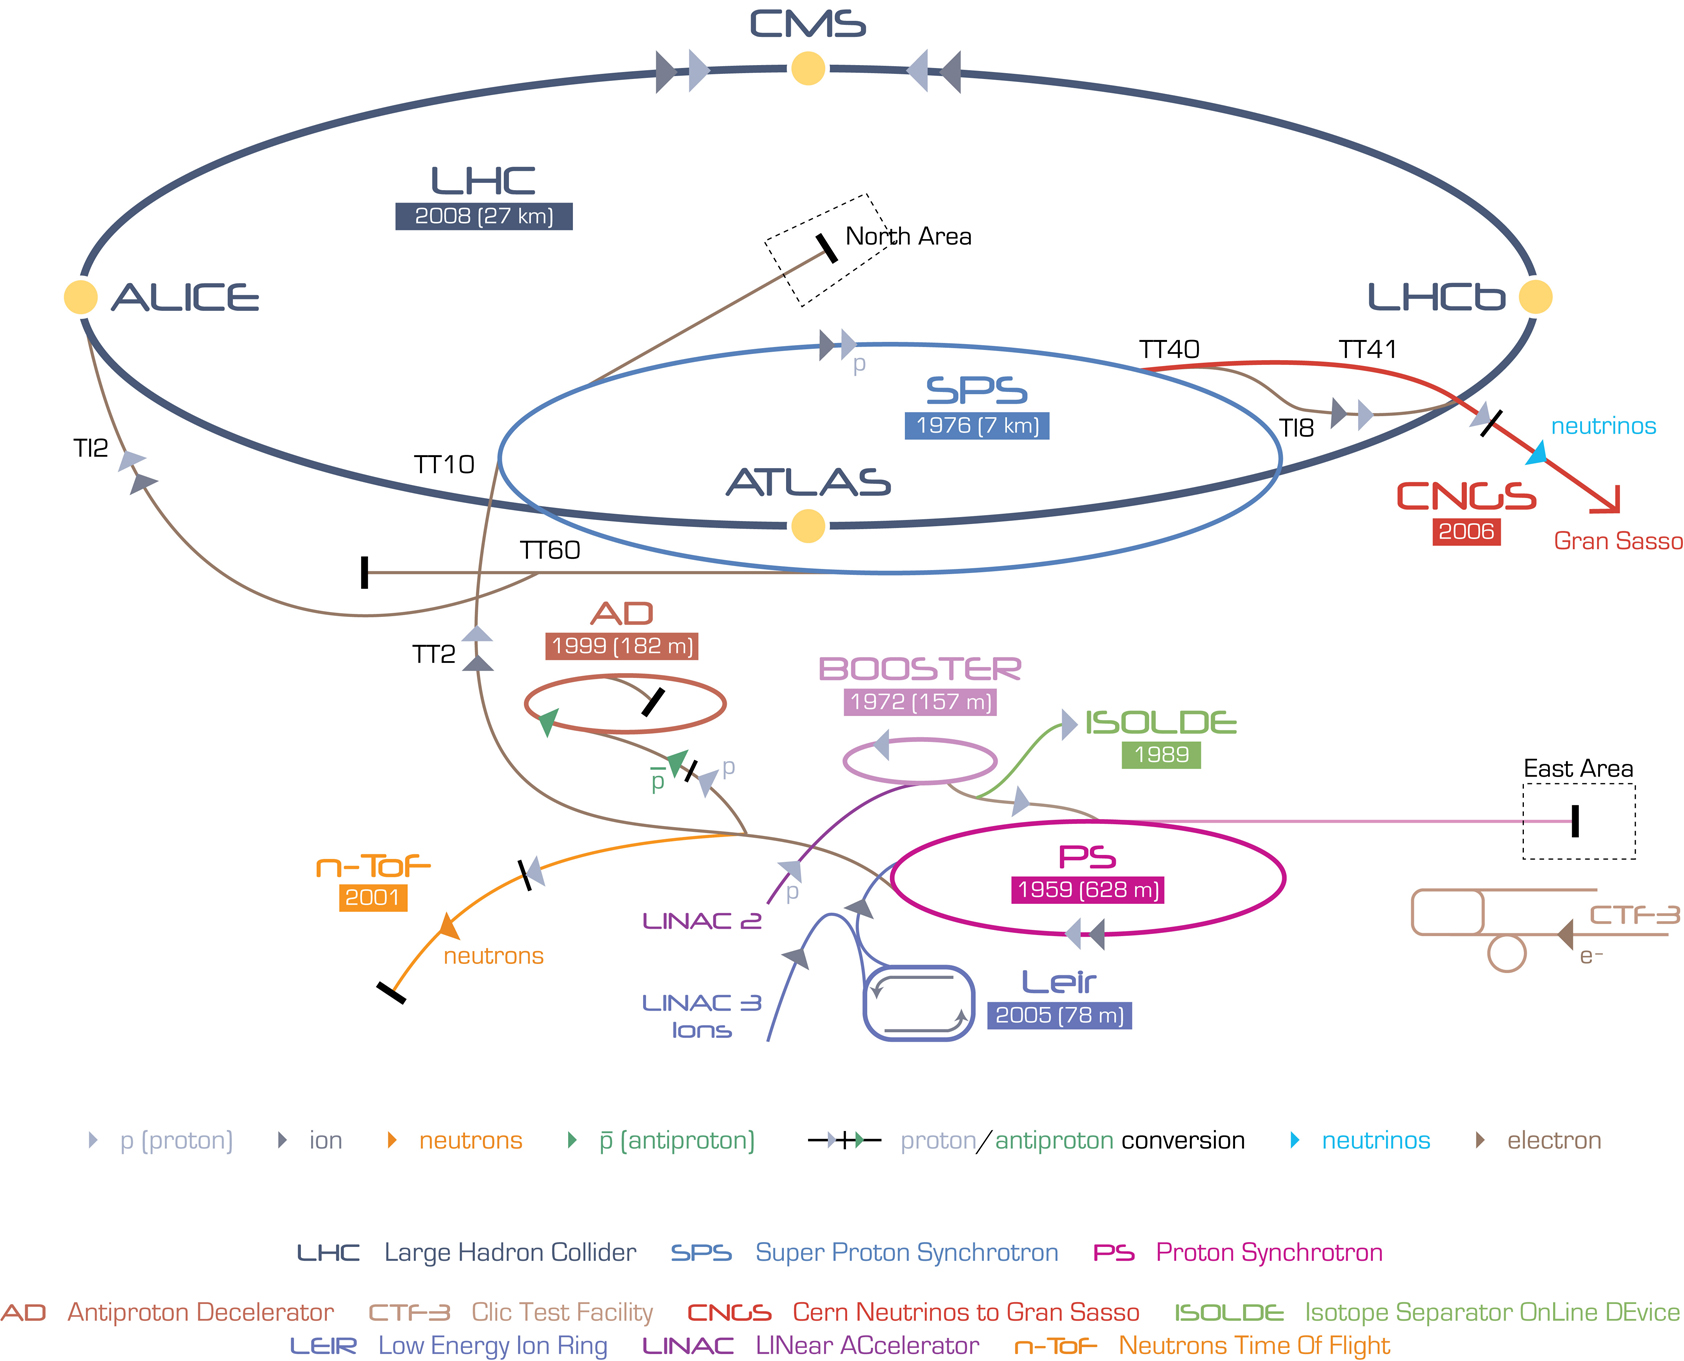
\includegraphics[width=0.8\textwidth]{Figures/LHC.jpg}
		%\rule{35em}{0.5pt}
	\caption[Schematics of Large Hadron Collider]{Schematics of Large Hadron Collider}
	\label{fig:LHC}
\end{figure}
%----------------------------------------------------------------------------------------
%	SECTION 1
%----------------------------------------------------------------------------------------

\section{Physics goals for the LHC}

The Standard model of elementary particles describes nicely all known particles and interactions, however there are still some unanswered questions. One of the major open questions was the existence of Higgs boson which was recently answered with the discovery of a new boson at 125 GeV. In order to be able to claim such a discovery, all known Standard model processes have to be well measured and the behavior of the experimental device has to be well understood. These requirements lead to many precision measurements which determined precisely cross sections, couplings, masses and other parameters within the Standard model. Any deviation from predicted values can be an evidence for the existence of physics beyond Standard model. One of the questions that remain open is the unification of fundamental forces. One attempt to achieve this goal is the theory of supersymmetry which predicts that each particle has its heavier supersymmetric partner and at high energies could unify strong and electroweak forces. If the theory of supersymmetry is correct, lightest supersymmetic particles would be stable and could be detected at the LHC. Such particle would also be a great candidate for the dark matter considering it would interact only weakly and as such would fit nicely into the present dark matter theories. On the other hand, the problem of matter-antimatter asymmetry could be addressed trying to discover why is the world built only of matter. Other theories that involve extra dimensions, bound states of quarks and leptons and other exotic models can be tested as well. Within LHCs heavy ion program, lead-lead and lead-proton collisions were performed in which a state called quark-gluon plasma is produced that resembles the conditions in the early universe. 
\par During the past few years, various models for new physics have been extensively tested, and new exclusion limits have been set. After three years of data taking at 7 and 8 TeV, and a shutdown period of two years, LHC is now almost ready to deliver collisions at record energies of 13 TeV which could hopefully show signs of new physics.        

%-----------------------------------
%	SECTION 2
%-----------------------------------

\section{Design of the LHC}

The LHC is located inside a 27 km tunnel, which lies between 45 m and 170 m below the ground surface and previously housed LEP accelerator. Beams circulating inside the LHC, collide at four interaction points. At each of these points, a detector has been built to record the products of particle collisions. This thesis was done using data collected with the CMS (Compact Muon Solenoid) detector \cite{Chatrchyan:2008aa}. Another detector with the same purpose but different design is the ATLAS (A Toroidal LHC Apparatus) detector located at the opposite side of the LHC ring \cite{Aad:2008zzm}. These two are so called multiple purpose particle detectors, which cover a wide range of physics topics, from searches for Higgs boson and supersymmetry to Standard model precision measurements. ALICE (A Large Ion Collider Experiment) is designed to study quark-gluon plasma from lead-lead collisions or lead-proton \cite{Aamodt:2008zz}. LHCb (LHC Beauty) is aimed towards B physics, by studying decays of B mesons \cite{Alves:2008zz}. Two other experiments TOTEM and LHCf are placed away from the interaction point to measure the collision products along the beam direction.
\par The LHC is made out of nearly 9600 different magnets, including dipoles, quadrupoles, sextupoles, octupoles, etc. The the largest portion of the accelerator is made out of 1232 dipoles. These magnets are made using superconducting niobium-titanium (NbTi) cables which undergo a phase transition to a supercondutive state at 9.2K. 
In order to achieve superconductivity and be able to withstand very high currents (11850 A), cables have to be cooled with superfluid helium to less than 2K creating large magnetic fields that in dipoles, which can reach 8.2T. These fields bend the proton beams around the ring. Other higher order magnets are used to focus and correct the beam. 
Two proton beams are counter-circulating inside a single cryogenic structure which requires opposite magnetic field direction for each of the beams in order to be steared along the same circumference. One of the LHC magnets is shown in Figure \ref{fig:LHC_mag} together with the drawing of the magnetic field inside the dipole. 
    
\begin{figure}[htbp]
	\centering
  		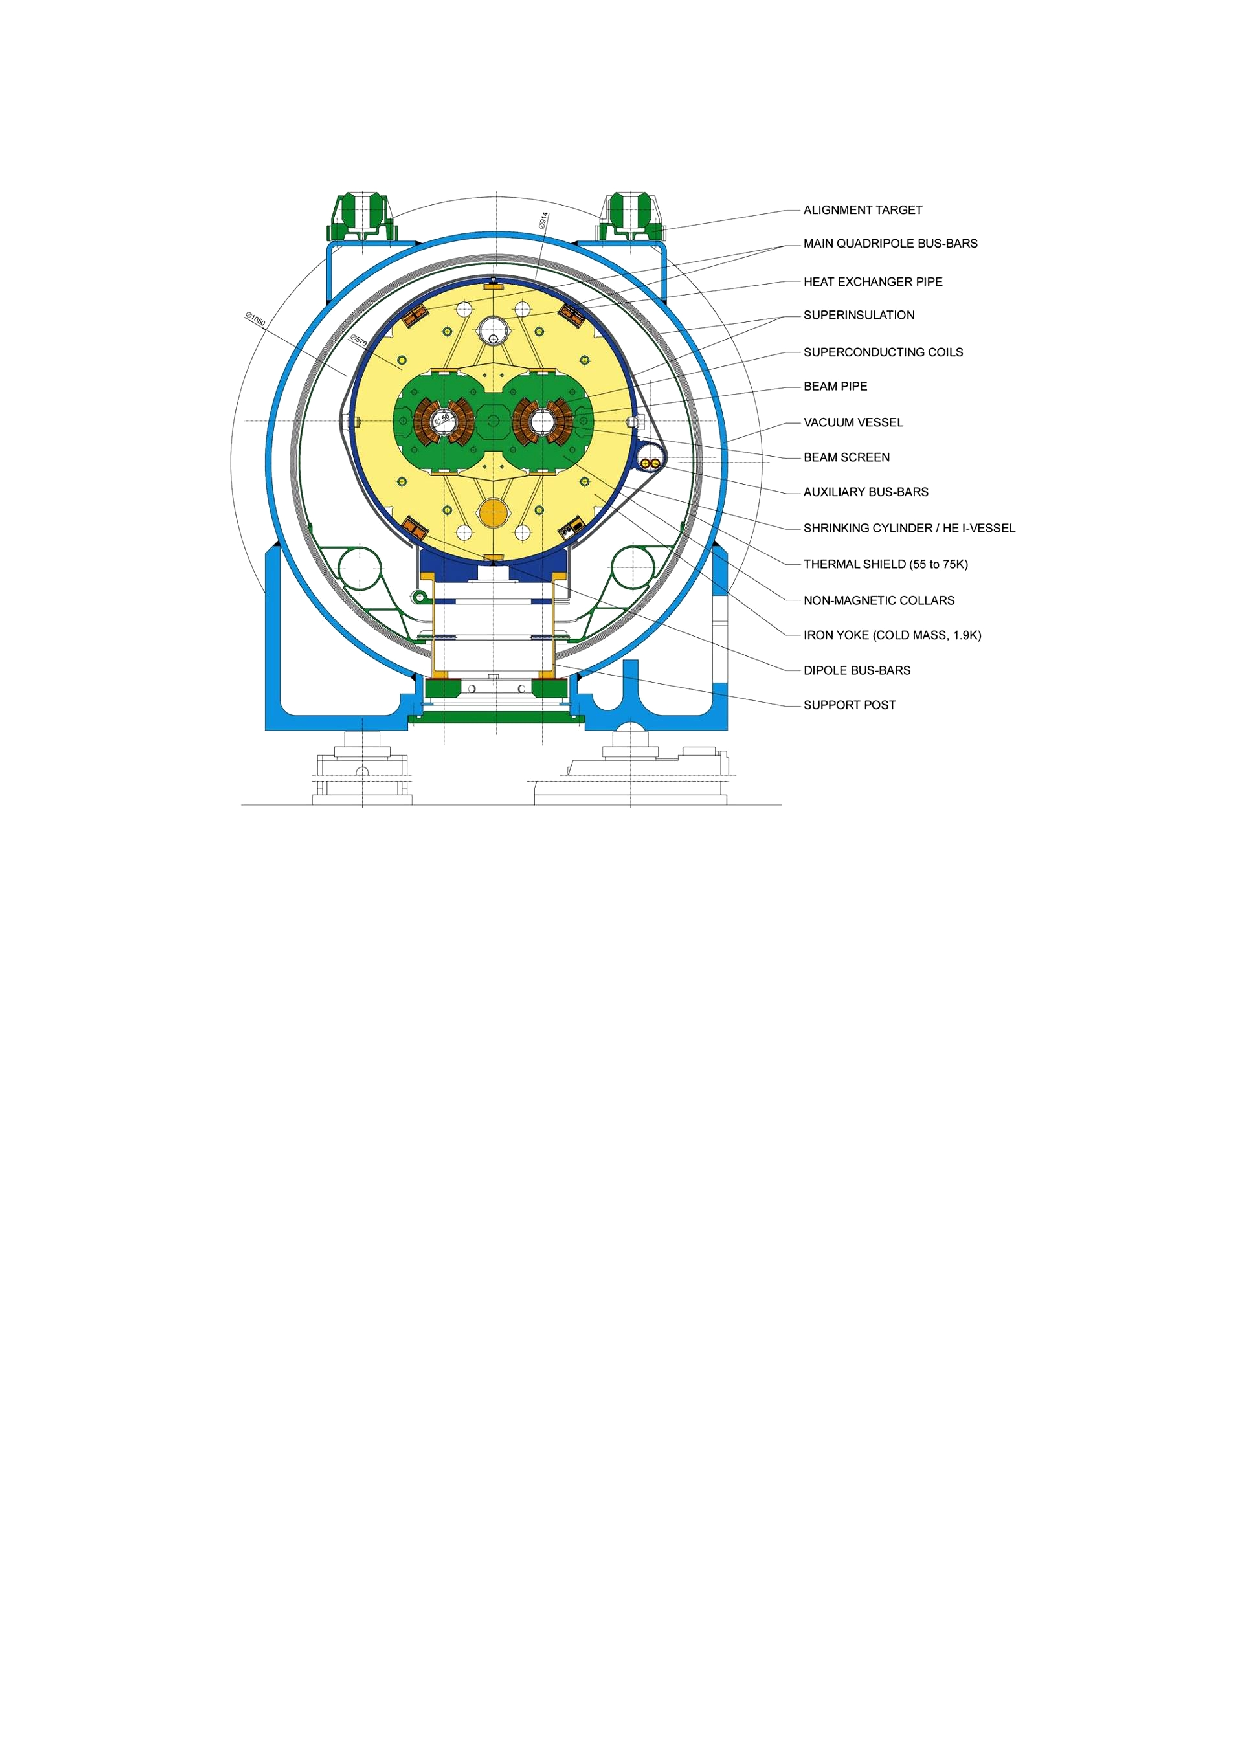
\includegraphics[width=0.6\textwidth]{Figures/LHC_magnet.pdf}
  		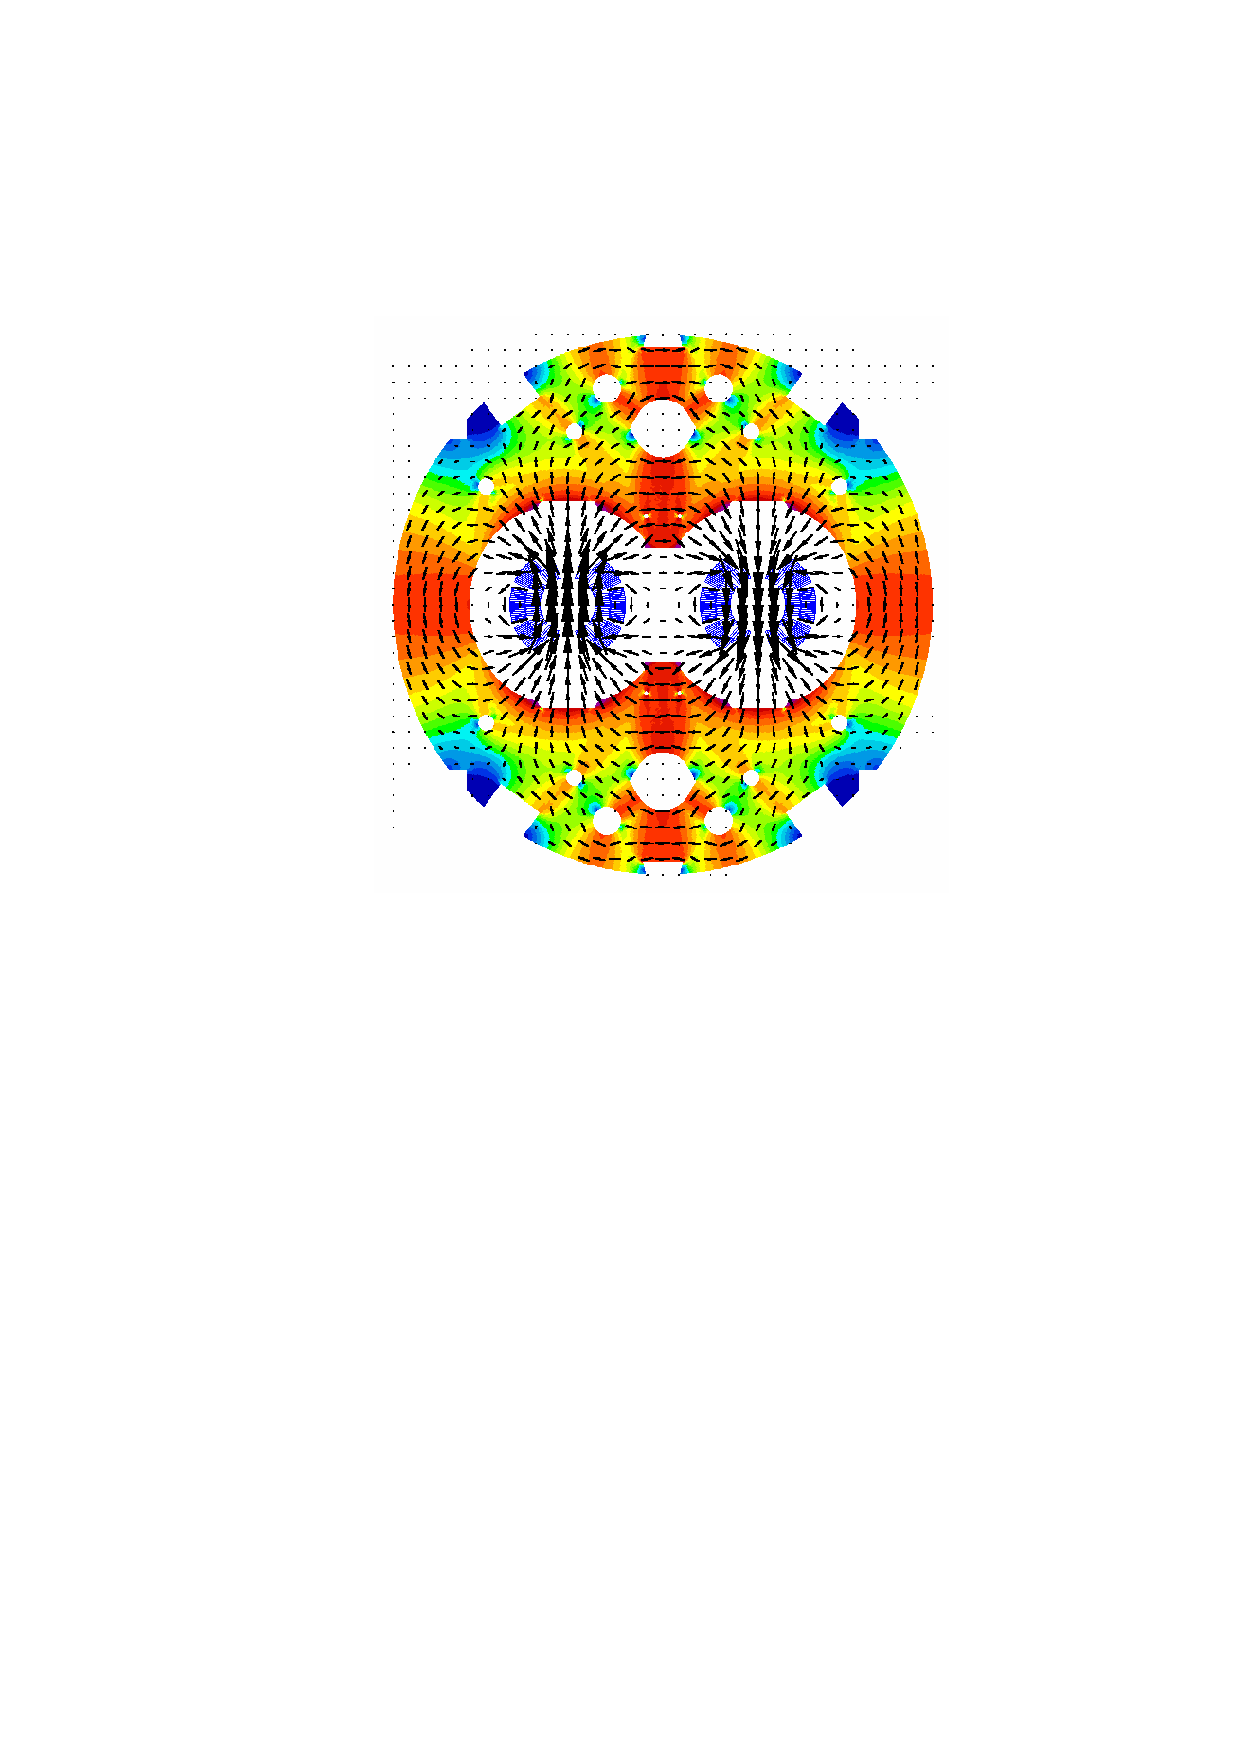
\includegraphics[width=0.39\textwidth]{Figures/LHC_MagVec.pdf}
	\caption[Schematics of dipole magnets]{Schematics of Dipole magnets \cite{Evans:2008zzb, Bruning:782076}}
	\label{fig:LHC_mag}
\end{figure}
 
\par Beams in the LHC are injected in series of bunches separated by a vacuum gaps, with each bunch having more than $10^{11}$ protons. Bunches are arranged in trains of 72 bunches with 25 ns spacing between them and 12 empty bunches between trains. Acceleration is provided by the radio frequency superconducting cavities (RF). It takes approximately 20 minutes for the beams to be accelerated from the injection at 450 GeV to the full beam energy. Moreover, RF chambers provide a small corrections of the order of $\sim 7$ keV per turn to the beam due to the energy loss from synchrotron radiation. After the acceleration, beams are tuned at the interaction points to achieve intersection. Peak collision rate of 40 MHz is achieved when collisions happen at every bunch crossing. Beams are squeezed to a transverse size of $\sim 17$ $\mu$m at the interaction point in order to maximize the probability of collision.  
    

%-----------------------------------
%	SECTION 3
%-----------------------------------

\section{Performance}

Since the start of the LHC in 2009, there were three years of machine operation, which yielded many physics results among which the discovery of Higgs boson should be highlighted. First year of operation was devoted to commissioning and understanding machine characteristics with the emphasis on safety and tests of the machine protection systems. In 2011 new energy and instantaneous luminosity records were reached. These numbers were increased once again in 2012 with center of mass energy going to 8 TeV.
\par High bunch intensity with 50 ns bunch spacing was used in order to get a good instantaneous luminosity performance. This came at a cost of high number of collisions in one bunch crossing (pile-up) which was around 12 collisions during 2011, and in some cases this number went as high as 20 interactions. With the increase of instantaneous luminosity in 2012, number of pile-up interactions was on the average around 30. Besides proton-proton collisions, LHC successfully delivered lead-lead ion runs in 2010 and 2011. primarily for the ALICE experiment, but also for CMS and ATLAS. On top of that, in the beginning of 2013 there was a successful proton-lead run performed for the first time. LHC design parameters together with the 2012 operations parameters are shown in Table \ref{tab:LHC_design}. Some of the highlights of Run 1 operation are shown in Table \ref{tab:LHC_highlights}.

\begin{table}[h]
\centering
  \caption{LHC performance in 2012 together with design performance\cite{Evans:2008zzb}}
	\label{tab:LHC_design}
  \begin{tabular}{ l  c  c }
      \hline
      \hline
      Parameter & Design value & Value in 2012 \\
      \hline
      Beam energy [TeV] & 7 & 4 \\
      Bunch spacing [ns] & 25 & 50 \\
      Number of bunches & 2808 & 1374 \\
      Protons per bunch & 1.15$\times 10^{11}$ & 1.6-1.7$\times 10^{11}$ \\
      Peak luminosity [cm$^{-2}$s$^{-1}$] & 1$\times 10^{34}$ & 7.7$\times 10^{33}$ \\
      Max. number of events per bunch crossing & 19 & $\approx 40$ \\
      Stored beam energy [MJ] & 362 & $\approx$ 140 \\
      \hline
      \hline 
  \end{tabular}
\end{table}

Luminosity ($L$) indicates the number of collisions per unit of time times the interaction cross section $\sigma$:
\begin{equation}
L=\frac{1}{\sigma}\frac{dN}{dt}
\end{equation}
Luminosity for collider experiments is connected to beam parameters:
\begin{equation}
L=\frac{n\cdot N^2 f}{A_{eff}}
\end{equation}
where $n$ is a number of bunches with $N$ protons inside, that are colliding with at the revolution frequency $f$ and effective beam area $A_{eff}$. The amount of data collected in a certain period of time is called total integrated luminosity and is defined as:
\begin{equation}
\mathcal{L} = \int L dt
\end{equation} 
During the Run 1 data taking period, the LHC delivered around 24fb$^{-1}$ of data (figure \ref{fig:LHC_lumi}) at the energy of 8 TeV with highest instantaneous luminosity of 8 $\cdot$ 10$^33$ cm$^{-2}$s$^{-1}$. Some of the LHC performance highlights are listed in table \ref{tab:LHC_highlights}.
\begin{table}[h]
\centering
  \caption{LHC performance highlights}
  \label{tab:LHC_highlights}
  \begin{tabular}{ l  c }
      \hline
      \hline
      Max. luminosity delivered in one fill & 237 pb$^{-1}$  \\
      Max. luminosity delivered in 7 days & 1.35 fb$^{-1}$  \\
      Longest time in stable beams (2012) & 22.8 hours \\
      Longest time in stable beams over 7 days & 91.8 hours (55$\%$) \\
      \hline
      \hline 
  \end{tabular}
\end{table}
\begin{figure}[htbp]
	\centering
		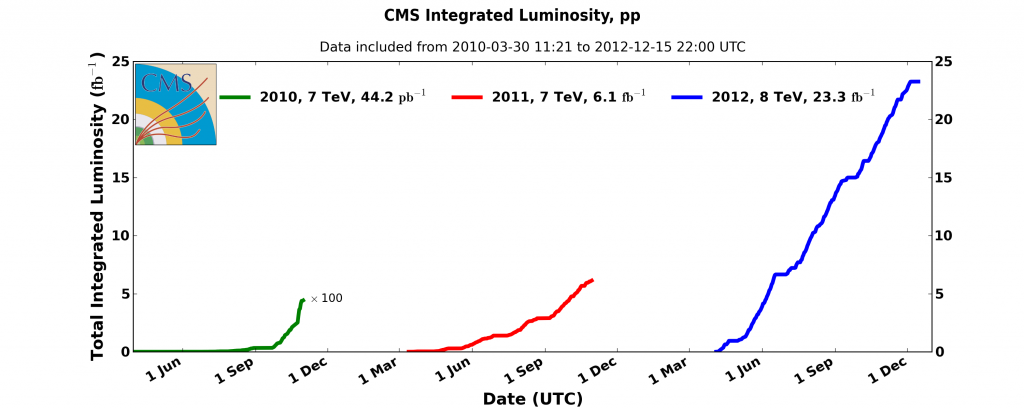
\includegraphics[width=\textwidth]{Figures/lumi.png}
		%\rule{35em}{0.5pt}
	\caption[Luminosity delivered to the CMS experiment]{Luminosity delivered to the CMS experiment}
	\label{fig:LHC_lumi}
\end{figure} 
\par Following a two year shutdown, LHC is anticipating operations at even higher energies of 6.5 TeV and later 7 TeV. The long term plan includes even higher peak luminosities, installation of the new injector complex and later the beginning of HL-LHC era. The timeline will, of course, be highly affected by the performance and results of the next run.